\documentclass{article}

\usepackage{fancyhdr}
\usepackage{graphicx}
\usepackage{ragged2e}
\usepackage{hyphenat}
\usepackage{hyperref}
\usepackage[margin=1.25in]{geometry}
\usepackage{xcolor}

\newcommand{\hangingcite}{\noindent\hangindent=0.5in\hangafter=1}

\graphicspath{{./../imgs/}}

\pagestyle{fancy}
\fancyhf{}

\fancyhead[L]{\color{lightgray}{\tiny ODIN Drone Concept of Operations (ConOps)}}
\fancyhead[R]{\color{lightgray}{\nouppercase{\tiny \leftmark}}}
\fancyfoot[C]{\thepage}

\begin{document}

\begin{titlepage}
    \begin{figure}
        \centering
        
\includegraphics[scale=1.25]{Bifrost_Logo.png}
    \end{figure}

    \vspace*{1cm}
    \justifying

    {\noindent\huge \textbf{\nohyphens{ODIN Drone Concept of \\ Operations (ConOps)}} \\}
    {\noindent\large \textbf{Version 2.0} \\}

    \vfill

    {\noindent\large \textbf{Prepared by:} \\}
    {\noindent\large \textbf{Bifröst Space Systems}}
\end{titlepage}

\tableofcontents
\newpage

\section{Summary/Mission Concept}
\vspace{0.5cm}

\begin{figure}[h]
    \centering
    \caption{ODIN Drone Mission Phases}
    \label{fig:ConOps_Graphic}
    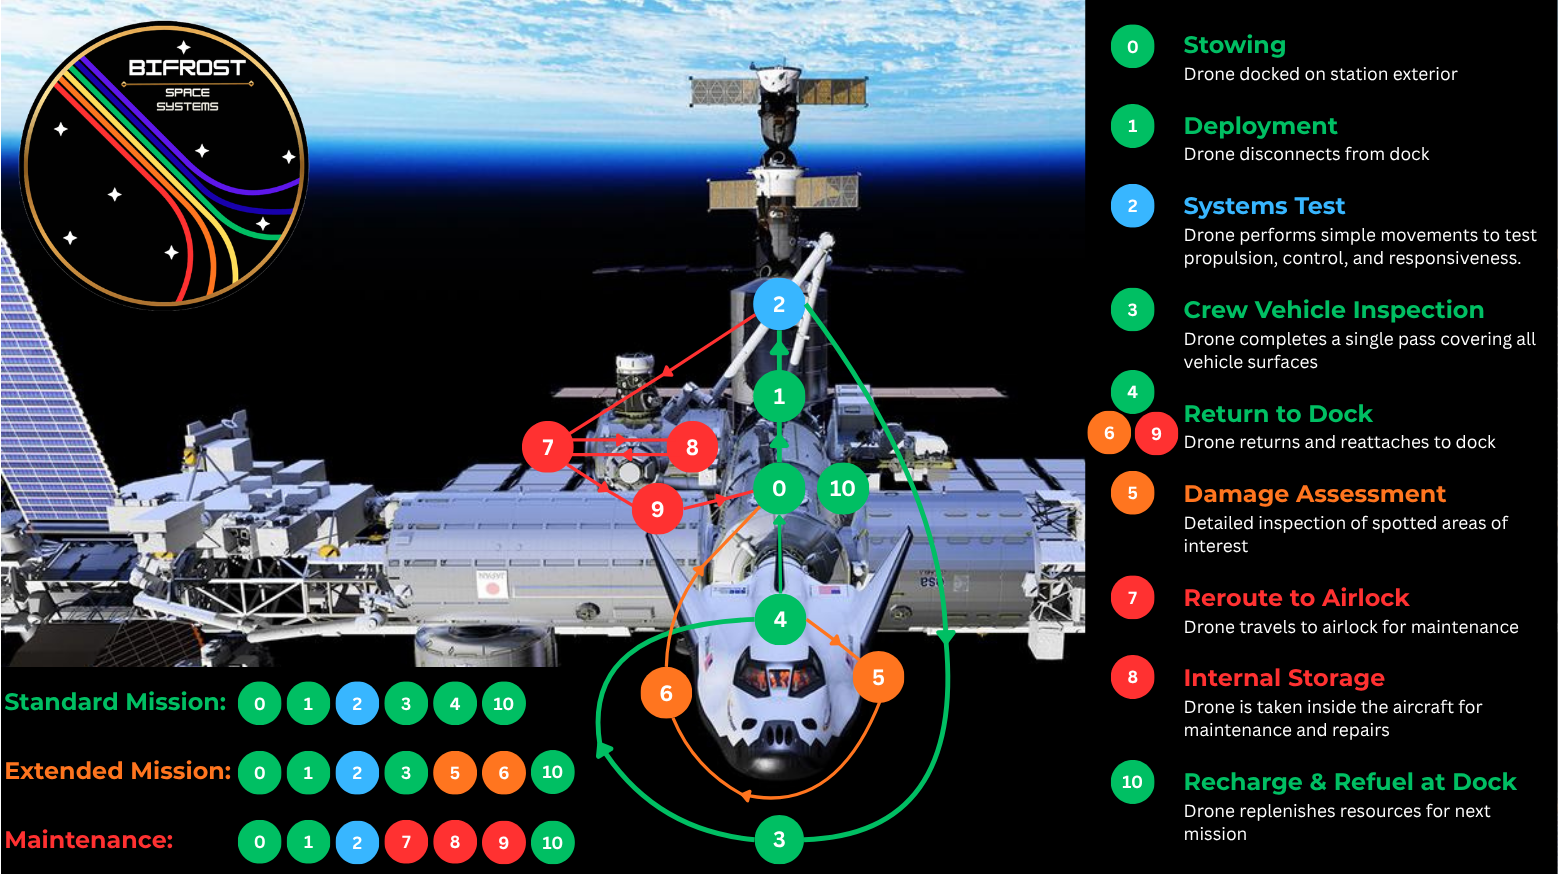
\includegraphics[width=\textwidth, keepaspectratio]{ConOps Graphic.png}
\end{figure}

\vspace{0.5cm}
\noindent The Observational Damage Inspector (ODIN) Drone will enhance the safety of all spacecraft launched from Earth and docked with space stations. Integrating its systems with the space station, ODIN will be piloted to conduct a non-destructive external scan of the docked spacecraft.

\vspace{\baselineskip}
\noindent The ODIN drone will undock from the space station, maneuver to the target spacecraft, and use a high-resolution camera to analyze the surface of the docked spacecraft, searching for any and all surface damage that may have been accrued during launch. Following this, the drone will return to the docking port and recharge. During the mission, astronauts aboard the space station and incoming spacecraft, NASA analysts, and business partners will all coordinate to ensure the safety of the spacecraft.  

\newpage

\section{Mission Phases}
The following sections describe the mission phases of the ODIN drone.

\subsection{Stowage/Pre-Use}
Initially turned off, conduct inspection (leaks, damage), (install fuel tank(s) and batter(ies) if stored separately), turn on, pre-flight checks.

\subsection{Flight Phase}
\subsubsection{Systems Test}
During all flight phases of ODIN, the first operation completed after undocking is a flight systems test. 
This test ensures that the control and propulsion systems are operating nominally. 
If anomalies are detected, the mission is re-routed, and the operations of \ref{subsubsec:Maintenance} are followed.

\subsubsection{Nominal Operations}
Following the systems test, ODIN progresses on its mission plan. 
The drone is navigated to the crew vehicle where a standard inspection of the vehicle is completed. 
If the first pass inspection is determined to be sufficient, the ODIN operators move on to \ref{subsubsec:Return}, else, \ref{subsubsec:Anomaly_Inspection} is followed. 

\subsubsection{Anomaly Inspection}
\label{subsubsec:Anomaly_Inspection}
If an anomaly is detected, the ODIN crew will return to the location of the anomaly to re-inspect this section. 
Once enough data is collected to determine the proper course of action for the crew vehicle, operators move to \ref{subsubsec:Return}. 

\subsubsection{Return}
\label{subsubsec:Return}
ODIN is piloted back to its stowage area where it is re-docked to the station. 

\subsubsection{Maintenance}
\label{subsubsec:Maintenance}
If an anomaly is detected in ODIN's systems, then the drone will be brought into the station for maintenance. 
If the anomalies are not critical for flight controls, ODIN can be piloted to an airlock for retrieval. 
If an anomaly is detected that is critical for flight control, case specific procedures will need to be followed to retrieve the drone and to ensure the safety of the crew and to protect the space station from damage. 
Once the drone is retrieved and brought into the station, repairs can be made to restore functionality to the ODIN drone.
Once ODIN's functionality is restored, the drone can then be returned to its dock where nominal operations can once again be conducted.

\subsection{Post-Use/Storage}
After a mission has been completed and ODIN has returned to its dock, a post-mission inspection is completed. 
After the inspection is complete, ODIN is powered off until next usage. 

\newpage
\section{Sub-System Overview}
\subsection{Structures}
The Structures team will be responsible for designing, modeling, and analyzing the structural components of the ODIN and its docking bay. The team will develop CAD models, evaluate structural loads and thermal effects, and integrate mounting features for all other sub systems. The team will seek a design that minimizes size and weight while maintaining structural strength, thermal control, subsystem integration, and maintenance access. Coordination with the materials sub-team will ensure that the design provides adequate strength and durability for ODIN’s lifetime. The team will also coordinate with all other subsystems to plan and resolve layout and attachment needs while providing access for maintenance.  

\subsubsection{Materials}
The Materials sub-team will be responsible for testing and selecting the most efficient materials for the various components aboard the ODIN. This process will include researching, testing, and implementing different materials and their best application. Factors such as weight, strength, durability, thermal/radiation resistance, and human factors are important for the success of the ODIN Mission. This sub-team will also serve as a backup to the structures team, assisting with designing and modeling ODIN and its docking bay. 

\subsection{Propulsion}
The propulsion system will provide the means for the drone to traverse the exterior of the space station.  The drone will use a propulsion system not yet decided to propel itself around the crew vehicle on a TBD route. All fuel or propellants needed for propulsion will be safely stored within the ODIN drone during missions. The propulsion system will work in conjunction with the control and communications systems to ensure the drone is responsive to human pilot input. While docked, the drone will be able to replenish any lost fuel or propellant to ready itself for its next mission. 

\subsection{Controls}
The control systems will be designed to execute various tasks, including monitoring imaging positions, maneuvering docking procedures, and promptly provide feedback in case of emergencies. For basic movement and maneuvers, the pilot will have command of the craft and provide input, while the control systems provide adequate feedback. In maneuvers such as docking, undocking, and inspection, the control systems will ensure the craft remains within the tolerances to successfully perform these operations. While in the imaging stages, controls will ensure the aircraft remains within the bounds to complete its imaging tasks. In emergency cases, such as when the craft is running low on resources or when communications are lost, the craft will initiate appropriate warnings to the pilot when necessary. 

\subsection{Power}
The power system onboard the ODIN drone will support all electronics within the drone, such as the camera, propellent control, and communications. The power system will be stored within the drone and will recharge when docked on the space station. Every full charge of the power supply will be enough to last one full mission, as well as longer in case of emergencies. This system will work in conjunction with all other systems, as it is dependent on structures, and supports propulsion, controls, and command.    

\subsection{Communications/Command}
The communication/command system will facilitate the astronauts' interactions with the ODIN drone. 
The system will utilize a radar system (TBD) to track ODIN's position and velocity. 
The communication/command system will also utilize a TBD camera for inspection in addition to providing a live feed for piloting ODIN.  
The communication/command system will have a radio control unit to allow the user to pilot ODIN and conduct vehicle inspection. 

\newpage
\section{References}
\vspace{0.5cm}
\hangingcite ``Appendix S: Concept of Operations Annotated Outline.'' \textit{NASA}, edited by Garrett Shea, National Aeronautics and Space Administration, 26 July 2023, \url{www.nasa.gov/reference/appendix-s-concept-of-operations-annotated-outline/}.

\vspace{0.5cm}
\hangingcite Gonzalez-Torres, Tomas. ``Concept of Operations / Mission Concept.'' \textit{AerE 4610 Modern Design Methodology with Astronautics Applications}, Iowa State University, Fall 2026. \textit{Canvas}, \url{canvas.iastate.edu}.

\vspace{0.5cm}
\hangingcite Sierra Nevada Corporation. ``Dream Chaser Docked to ISS.'' \textit{Space.com}, 29 Oct. 2012, \url{www.space.com/14446-photos-dream-chaser-space-plane/6.html}.
\end{document}